\section{Methodology}

\subsection{Testing Environment}

We used the following computational environment for our experiments:
\begin{itemize}
    \item OS: Linux 6.8.0-64-generic
    \item CPU: Intel Xeon Gold 6130 2.10GHz - 32 cores / 64 threads
    \item GPU: NVIDIA Quadro P5000 - 16GB VRAM
    \item RAM: 512GB
    \item DISK: 7.6TB 
\end{itemize}
The hardware was provided for research purposes by Universidade de São Paulo. The choice of this environment was motivated by the availability of a high-performance GPU and large quantities of RAM necessary for handling large language models.

We used the following tools and libraries:
\begin{itemize}
    \item Python 3.12.3
    \item PyTorch 2.8.0 \cite{Paszke2019}
    \item Transformers 4.56.2 \cite{Wolf2019}
    \item Hugging Face Hub 0.35.0 \cite{HuggingFaceHub}
    \item Numpy 2.2.6
    \item Pandas 2.3.2
    \item Pysr 1.5.9
    \item SciPy 1.16.1
    \item Matplotlib 3.10.6
    \item Seaborn 0.13.2 \cite{Waskom2021}
    \item CUDA Toolkit 12.6
\end{itemize}
The choice of versions was motivated by compatibility with our computational environment GPU.

\subsection{Model Selection}

Due to the wide availability of open models combined with the ease of accessing them through the Transformers library \cite{Wolf2019} and Hub library \cite{HuggingFaceHub}, \textbf{Hugging Face} was chosen as the source for model selection in this study.

Hugging Face is a platform that hosts a variety of machine learning models, datasets, and tools. It is widely used in the AI research community for sharing and collaborating on machine learning projects \cite{HuggingFaceResearchGate, HuggingFaceMain}. Other platforms such as Ollama \cite{Ollama} were considered, but ultimately not chosen due to the limited number of models and lack of company diversity. 

Model selection proceeded in two stages:

\begin{enumerate}
    \item First, we identified major technology companies by market capitalization that publish openly released language models. The companies considered were \textbf{OpenAI}, \textbf{Google}, \textbf{Meta}, and \textbf{Microsoft}.
    \item Second, for each company we compiled a candidate set consisting of every model that satisfied the following criteria:
    
        \begin{itemize}
            \item Must be available on the Hugging Face platform on the official company account.
            \item The model is a transformer-based language model.
            \item Model weights are publicly accessible (open weights), including models released behind
            gated access.
            \item The model is text-only (no multimodal image/audio inputs).
            \item The model is an original base model rather than a task-specific fine-tuned variant.
            \item The total parameter count is below 150 billion. This upper bound was imposed due to
            hardware and inference limitations in the computational environment used for our experiments.
            \item The model is supported by the Hugging Face Transformers library \cite{Wolf2019} (i.e., it can be
            instantiated via the AutoModel utility), which ensures consistent loading and
            preprocessing across the candidate set.
            \item There is at least one publicly available benchmark result for the model among the selected benchmarks (section \ref{sec:benchmark_selection}).
        \end{itemize}

\end{enumerate}

The final selection of models used in this study is listed in Table \ref{tab:selected_models}.

\begin{table}[H]
    \begin{tabular}{p{0.24\linewidth} p{0.24\linewidth} p{0.24\linewidth} p{0.24\linewidth}}
        \hline
        Meta & Google & Microsoft & OpenAI \\
        \hline
        meta-llama/Llama-4-Scout-17B-16E & google/gemma-3-27b-pt & microsoft/Phi-4-mini-reasoning & openai/gpt-oss-120b \\
        meta-llama/Llama-3.2-3B & google/gemma-3-12b-pt & microsoft/Phi-4-reasoning & openai/gpt-oss-20b \\
        meta-llama/Llama-3.2-1B & google/gemma-3-4b-pt & microsoft/Phi-4-reasoning-plus & openai-community/gpt2-xl \\
        meta-llama/Llama-3.1-70B & google/gemma-3-1b-pt & microsoft/phi-4 & openai-community/gpt2-large \\
        meta-llama/Llama-3.1-8B & google/gemma-3-270m & microsoft/phi-2 & openai-community/gpt2-medium \\
        meta-llama/Meta-Llama-3-70B & google/gemma-2-27b & microsoft/phi-1\_5 & openai-community/gpt2 \\
        meta-llama/Meta-Llama-3-8B & google/gemma-2-9b & microsoft/phi-1 & \\
        meta-llama/Llama-2-70b-hf & google/gemma-2-2b &  & \\
        meta-llama/Llama-2-13b-hf & google/gemma-7b &  & \\
        meta-llama/Llama-2-7b-hf & google/gemma-2b &  & \\
            & google/recurrentgemma-9b &  & \\
            & google/recurrentgemma-2b &  & \\
        \hline
    \end{tabular}
    \caption{Selected language models included in this study.}
    \label{tab:selected_models}
\end{table}

\begin{tcolorbox}[colback=gray!10, colframe=black, boxrule=1pt, rounded corners]
    \textbf{Meta Models}:
    \cite{MetaLlama4Scout}
    \cite{MetaLlama3.2-3B}
    \cite{MetaLlama3.2-1B}
    \cite{MetaLlama3.1-70B}
    \cite{MetaLlama3.1-8B}
    \cite{MetaLlama3-70B}
    \cite{MetaLlama3-8B}
    \cite{MetaLlama2-70b}
    \cite{MetaLlama2-13b}
    \cite{MetaLlama2-7b}

    \textbf{Google Models}:
    \cite{GoogleGemma3-27b}
    \cite{GoogleGemma3-12b}
    \cite{GoogleGemma3-4b}
    \cite{GoogleGemma3-1b}
    \cite{GoogleGemma2-27b}
    \cite{GoogleGemma2-9b}
    \cite{GoogleGemma2-2b}
    \cite{GoogleGemma-7b}
    \cite{GoogleGemma-2b}
    \cite{GoogleRecurrentGemma-9b}
    \cite{GoogleRecurrentGemma-2b}

    \textbf{Microsoft Models}:
    \cite{MicrosoftPhi4-mini-reasoning}
    \cite{MicrosoftPhi4-reasoning}
    \cite{MicrosoftPhi4-reasoning-plus}
    \cite{MicrosoftPhi4}
    \cite{MicrosoftPhi2}
    \cite{MicrosoftPhi1-5}
    \cite{MicrosoftPhi1}

    \textbf{OpenAI Models}:
    \cite{OpenAIGPT-oss-120b}
    \cite{OpenAIGPT-oss-20b}
    \cite{OpenAIGPT2-xl}
    \cite{OpenAIGPT2-large}
    \cite{OpenAIGPT2-medium}
    \cite{OpenAIGPT2}
\end{tcolorbox}

\subsection{LMC Complexity}
\label{sec:lmc_complexity}

    According to \cite{LopezRuiz1995}, LMC Statistical Complexity is the product of two other measures: Disequilibrium and Shannon entropy. It captures both the structured and unstructured aspects of the distribution:
    \[ C_{LMC} = H \times D \]

    Disequilibrium measures how far a probability distribution is from being uniform, quantifying the "order" or structure in the data. It is calculated as:
    \[ D = \sum_{i=1}^{n} \left(p_i - \frac{1}{n}\right)^2 \]

    Shannon entropy measures the amount of uncertainty or randomness in a probability distribution. The normalized Shannon entropy is given by:
    \[ H = -K \sum_{i=1}^{n} p_i \log p_i \]

    The values \( p_i \) represent the probabilities associated with each state \( i \) in the distribution, and \( n \) is the total number of states. K is a positive constant and, in our case, is set to 1 for simplicity. K can be changed later since \( C_{LMC} = (-K \sum_{i=1}^{n} p_i \log p_i)  \times D \) is equivalent to \( C_{LMC} = K \times (- \sum_{i=1}^{n} p_i \log p_i)  \times D \).

    \subsubsection{Reading Model Weights}

        Model weights are fetched using the Hugging Face Hub library \cite{HuggingFaceHub} and loaded using the Transformers library \cite{Wolf2019}. For each selected model, we instantiate the model using the \textbf{AutoModel} utility, which automatically handles model architecture loading and weight initialization. 

        The models are loaded entirely into the main memory instead of a GPU since the amount of VRAM available in the computational environment is insufficient for larger models $(> 70 \text{ billion parameters})$. Other problems such as handling symbolic tensors also motivated this decision.

        Using the main memory is considerably slower than using a GPU, but allows us to work with larger models without running into memory limitations. Since we had a large amount of RAM, we decided to cast all the model weights to float32 during the AutoModel instantiation as CPUs generally handle this format natively and, as a consequence, make calculations faster.
        
        Once loaded, we extract all the parameters from the model using the \texttt{named\_parameter()} method provided by the Transformers library. This method returns an iterator over all model parameters, each parameter being represented as a tensor. 

        We then flatten each tensor into a one-dimensional array and store it in a list. Each array is labeled in one of the following \textbf{weight-type categories}:
        \begin{itemize}
            \item Bias: if 'bias' is in the parameter name
            \item Norm: if 'norm' is in the parameter name
            \item Embedding: if 'embed' is in the parameter name
            \item Other: all other weights
        \end{itemize}

        These categories are the most common types of weights found in this architecture and will be used later as another dimension of analysis. 
        
        The choice of also analyzing by weight type is motivated by the fact that different weight types may exhibit different statistical properties and, as a consequence, different complexity characteristics. Studies such as the already cited OpenAI's \cite{Kaplan2020} take into account different weight types when analyzing scaling laws.

    \subsubsection{Filtering}

        Casting different encoding formats to float32 may introduce rounding errors that manifest as extreme outliers in the weight distribution. This is rare (approximately 10 to 30 values in 100 billion) but can be problematic for our next step: histogram construction (section \ref{sec:data_discretization}), since the number of bins will be affected by the range of values in the data. The reasons for those rounding errors could not be fully investigated within the scope of this work, but they are likely related to floating point rounding errors.

        To mitigate the impact of outliers, we will apply a value removal approach. This process filters the data to retain only values within a configurable range centered around the mean:

        \[ \text{lower bound} = \mu - \sigma_{\text{filter}} \cdot \sigma \]
        \[ \text{upper bound} = \mu + \sigma_{\text{filter}} \cdot \sigma \]

        where \( \mu \) is the data mean, \( \sigma \) is the data standard deviation, and \( \sigma_{\text{filter}} \) is a configurable parameter that controls the filtering strength. Values falling outside this range are excluded from further analysis. 

        It is not trivial to choose the best value for \( \sigma_{\text{filter}} \). A very low value may remove important parts of the distribution, while a very high value may not effectively mitigate the outlier problem. For this reason, we will experiment with different values of \( \sigma_{\text{filter}} \) and analyze how they affect the final complexity results. As a consequence, this becomes yet another dimension of analysis in our study.

        The values of \( \sigma_{\text{filter}} \) tested will be: \textbf{0.125}, \textbf{0.25}, \textbf{0.5}, \textbf{1}, \textbf{2}, \textbf{3}, \textbf{4}, \textbf{5}, \textbf{10}, \textbf{20}. The choice of \( \sigma_{\text{filter}} \) that will be used as the data's filtering option for the next steps is the one that: 
        \begin{enumerate}
            \item most reduces the bin count compared to the unfiltered data; 
            \item has the least amount of filtering or, in other words, the highest value of \( \sigma_{\text{filter}} \) among the ones chosen in the first criterion.
        \end{enumerate}

    \subsubsection{Data Discretization and Histogram}
    \label{sec:data_discretization}

        To compute the LMC complexity of a finite array of floating-point numbers, we first construct a histogram to discretize the data into a probability distribution. That's justified as the chance of finding two exact numbers is extremely low and, as a consequence, it is hard to determine the probability of each value. 
        
        We will call the set of all data points as \( S \), the total amount of data points as \( N \) and the number of bins they will be distributed into as \( n \). The probabilities \( p_i \) are then calculated as \( p_i = \frac{f_i}{N} \) where \( f_i \) is the frequency count of data points in bin \( i \).

        As expected, this approach revisits a classic issue in histogram-based analysis: the choice of the number of bins \( n \) will impact the resulting probability distribution, which is specially problematic to the LMC complexity measure; variations in \( n \) can cause significant fluctuations in the final result. Selecting an inappropriate amount may produce misleading values, either by oversimplifying the distribution (too few bins) or by introducing noise (too many bins). 

        There are a variety of methods to determine \( n \) in a histogram, most of them with their own advantages and disadvantages. Commonly used methods such as \textbf{Sturges' formula} \cite{Sturges1926} and \textbf{Rice Rule} \cite{RiceRule} rely only on the number of data points, while others like \textbf{Scott's normal reference rule} and \textbf{Freedman-Diaconis' choice} also take into account the data distribution by using standard deviation and interquartile range, respectively \cite{Knuth2006}.   

        We chose to use the \textbf{Freedman-Diaconis' choice} as it adapts better to our needs. This is justified since \( N \) often consists of billions of numbers, and the distribution, although mostly concentrated between -1 and 1, can become sparse due to outliers and, as a consequence, require a larger number of bins to capture its characteristics accurately. The Freedman-Diaconis rule helps mitigate the influence of outliers by using the interquartile range \( IQR \) to determine bin width \( h \). The rule is defined as follows \cite{FreedmanDiaconis1981}:

        \[ h = \frac{2 \times IQR}{N^{1/3}} \]

        where IQR is the interquartile range of the data which is calculated as \( Q3 - Q1 \), \( Q3 \) and \( Q1 \) are the values at the 75th and 25th percentiles in the data, respectively. Since \( N \) is very large, the percentiles are computed based on a random sample of 100000 data points to reduce computational cost. The sample size was determined empirically to be large enough to provide stable estimates of the percentiles, the final number of bins showed no variance between tests.

        The number of bins \( n \) can then be calculated as:

        \[ n = \frac{\max(S) - \min(S)}{h} \]

        Finally, we can use the already filtered data and the calculated \( n \) to build a histogram using a simple function provided by PyTorch \cite{Paszke2019}. Then, compute the probabilities \( p_i \) for each bin \( i \).

    \subsubsection{Complexity Calculation}

        With the probabilities \( p_i \) computed from the histogram, we can now calculate the LMC complexity \( C_{LMC} \) using the formulas provided in the beginning of section \ref{sec:lmc_complexity}. This involves calculating the Disequilibrium \( D \) and the Shannon entropy \( H \) using the probabilities, and then multiplying them to obtain the final complexity measure \( C_{LMC} \).

\subsection{Inference Capability}

    Often called model performance, inference capability refers to how well a trained neural network performs on unseen data. This is typically measured using various metrics depending on the specific task the model is designed for. 
    
    In the previously cited research paper by OpenAI \cite{Kaplan2020}, performance was associated with test cross-entropy loss. This metric quantifies the difference between the predicted probability distribution output by the model and the true distribution of the target labels. Lower cross-entropy loss values indicate better model performance, as they reflect a closer alignment between predictions and actual outcomes.

    Unfortunately, not all models we intend to analyze have publicly available training and test data. It's also not possible to run models in a training setting due to performance limitations of the computational environment available. Therefore, we will have to rely on imperfect proxies for performance such as \textbf{benchmarks}.

    \subsubsection{Benchmark Selection}
    \label{sec:benchmark_selection}

        Benchmarks are standardized tests designed to evaluate the performance of machine learning models across various tasks. They provide a common ground for comparison by measuring how well different models perform on the same datasets using predefined metrics. 
        
        According to \cite{Owen2024}, benchmarks such as the famous MMLU, correlate fairly well with the predicted test loss determined by scaling laws, making them suitable proxies.

        They are, however, not perfect. Some benchmarks may fail to capture all aspects of a model's capabilities, leading to an incomplete assessment of performance. Other problems such as Data Contamination \cite{Magar2022} can influence the validity of results and make it hard to fairly compare models made in different times. It is also hard to find benchmarks that are widely reported for all models we intend to analyze.

        A nice proposal for future research to avoid the problems cited above would involve training a model from scratch twice: optimizing it initially for minimal loss and then for minimal loss + maximum LMC complexity, then comparing the results. This is however out of the scope of this work.

        The benchmark selection followed three main heuristics:
        \begin{itemize}
            \item \textbf{Relevance}: The benchmark should be widely recognized and accepted in the machine learning community, e.g., used in major research papers.
            \item \textbf{Generality}: It should cover a range of tasks and data types to provide an assessment of model performance across different scenarios, that is, not being specialized in one task.
            \item \textbf{Availability}: The benchmark results should be publicly available. Benchmarks that cover more of the selected models were preferred.
        \end{itemize}

        Based on those heuristics, the benchmarks selected were:
        \begin{itemize}
            \item \textbf{MMLU (5-shot)}: Massive Multitask Language Understanding, a benchmark that tests models across 57 tasks spanning various subjects and difficulty levels. Widely used to evaluate LLMs \cite{Hendrycks2020}.

            \item \textbf{MMLU-Pro (5-shot)}: An enhanced version of MMLU that includes additional tasks and updated datasets to provide a better evaluation \cite{MMPro2024}.
            
            \item \textbf{OpenLLM (Average)}: A benchmark suite that evaluates models on a variety of tasks, including language understanding, generation, and reasoning. It aggregates results from multiple datasets to provide an overall performance score \cite{Myrzakhan2024}.
            
            \item \textbf{LMArena (Score)}: An online platform where users can submit questions and receive responses from two anonymous large language models (LLMs), then vote on which answer they prefer, helping to crowdsource human preferences for evaluating and ranking LLMs. Its evaluation works by collecting thousands of pairwise comparisons from users, using the Bradley-Terry system to estimate win rates and compute rankings/scores. \cite{Chiang2024}.
        \end{itemize}

    \subsubsection{Benchmark Collection Procedure}

        Benchmark values were manually collected from multiple sources, in the following order of priority:
        \begin{enumerate}
            \item Official \textit{Hugging Face} model pages
            \item Original research papers
            \item Official websites
            \item Third-party websites
        \end{enumerate}

        \begin{tcolorbox}[colback=gray!10, colframe=black, boxrule=1pt, rounded corners]
            \textbf{Meta Models}: 
            \cite{MetaLlama4Scout}, 
            \cite{MetaLlama3.2-3B}, 
            \cite{MetaLlama3.2-1B}, 
            \cite{MetaLlama3.1-70B}, 
            \cite{MetaLlama3.1-8B}, 
            \cite{MetaLlama3-70B}, 
            \cite{MetaLlama3-8B}, 
            \cite{MetaLlama2-70b}, 
            \cite{MetaLlama2-13b}, 
            \cite{MetaLlama2-7b}
            
            \textbf{Google Models}: 
            \cite{GoogleGemma3-27b}, 
            \cite{GoogleGemma3-12b}, 
            \cite{GoogleGemma3-4b}, 
            \cite{GoogleGemma3-1b}, 
            \cite{GoogleGemma2-27b}, 
            \cite{GoogleGemma2-9b}, 
            \cite{GoogleGemma2-2b}, 
            \cite{GoogleGemma-7b}, 
            \cite{GoogleGemma-2b}, 
            \cite{GoogleRecurrentGemma-9b}, 
            \cite{GoogleRecurrentGemma-2b}
            
            \textbf{Microsoft Models}: 
            \cite{MicrosoftPhi4-mini-reasoning}, 
            \cite{MicrosoftPhi4-reasoning}, 
            \cite{MicrosoftPhi4-reasoning-plus}, 
            \cite{MicrosoftPhi4}, 
            \cite{MicrosoftPhi2}, 
            \cite{MicrosoftPhi1-5}, 
            \cite{MicrosoftPhi1}, 
            \cite{Phi1.5}, 
            \cite{Phi2Blog}
            
            \textbf{OpenAI Models}: 
            \cite{OpenAIGPT-oss-120b}, 
            \cite{OpenAIGPT-oss-20b}, 
            \cite{OpenAIGPT2-xl}, 
            \cite{OpenAIGPT2-large}, 
            \cite{OpenAIGPT2-medium}, 
            \cite{OpenAIGPT2}, 
            \cite{OpenAIOpenModels},
            
            \textbf{Additional References}: 
            \cite{HuggingFaceMain}, 
            \cite{Ollama},
            \cite{LLMExplorer}, 
            \cite{RankedAGI},
        \end{tcolorbox} 

        If more than one source was available for the same model and benchmark, the one with higher priority was chosen. Not all models had results available for all benchmarks. Figure \ref{fig:benchmark_availability} shows the availability matrix.

        \begin{figure}[H]
            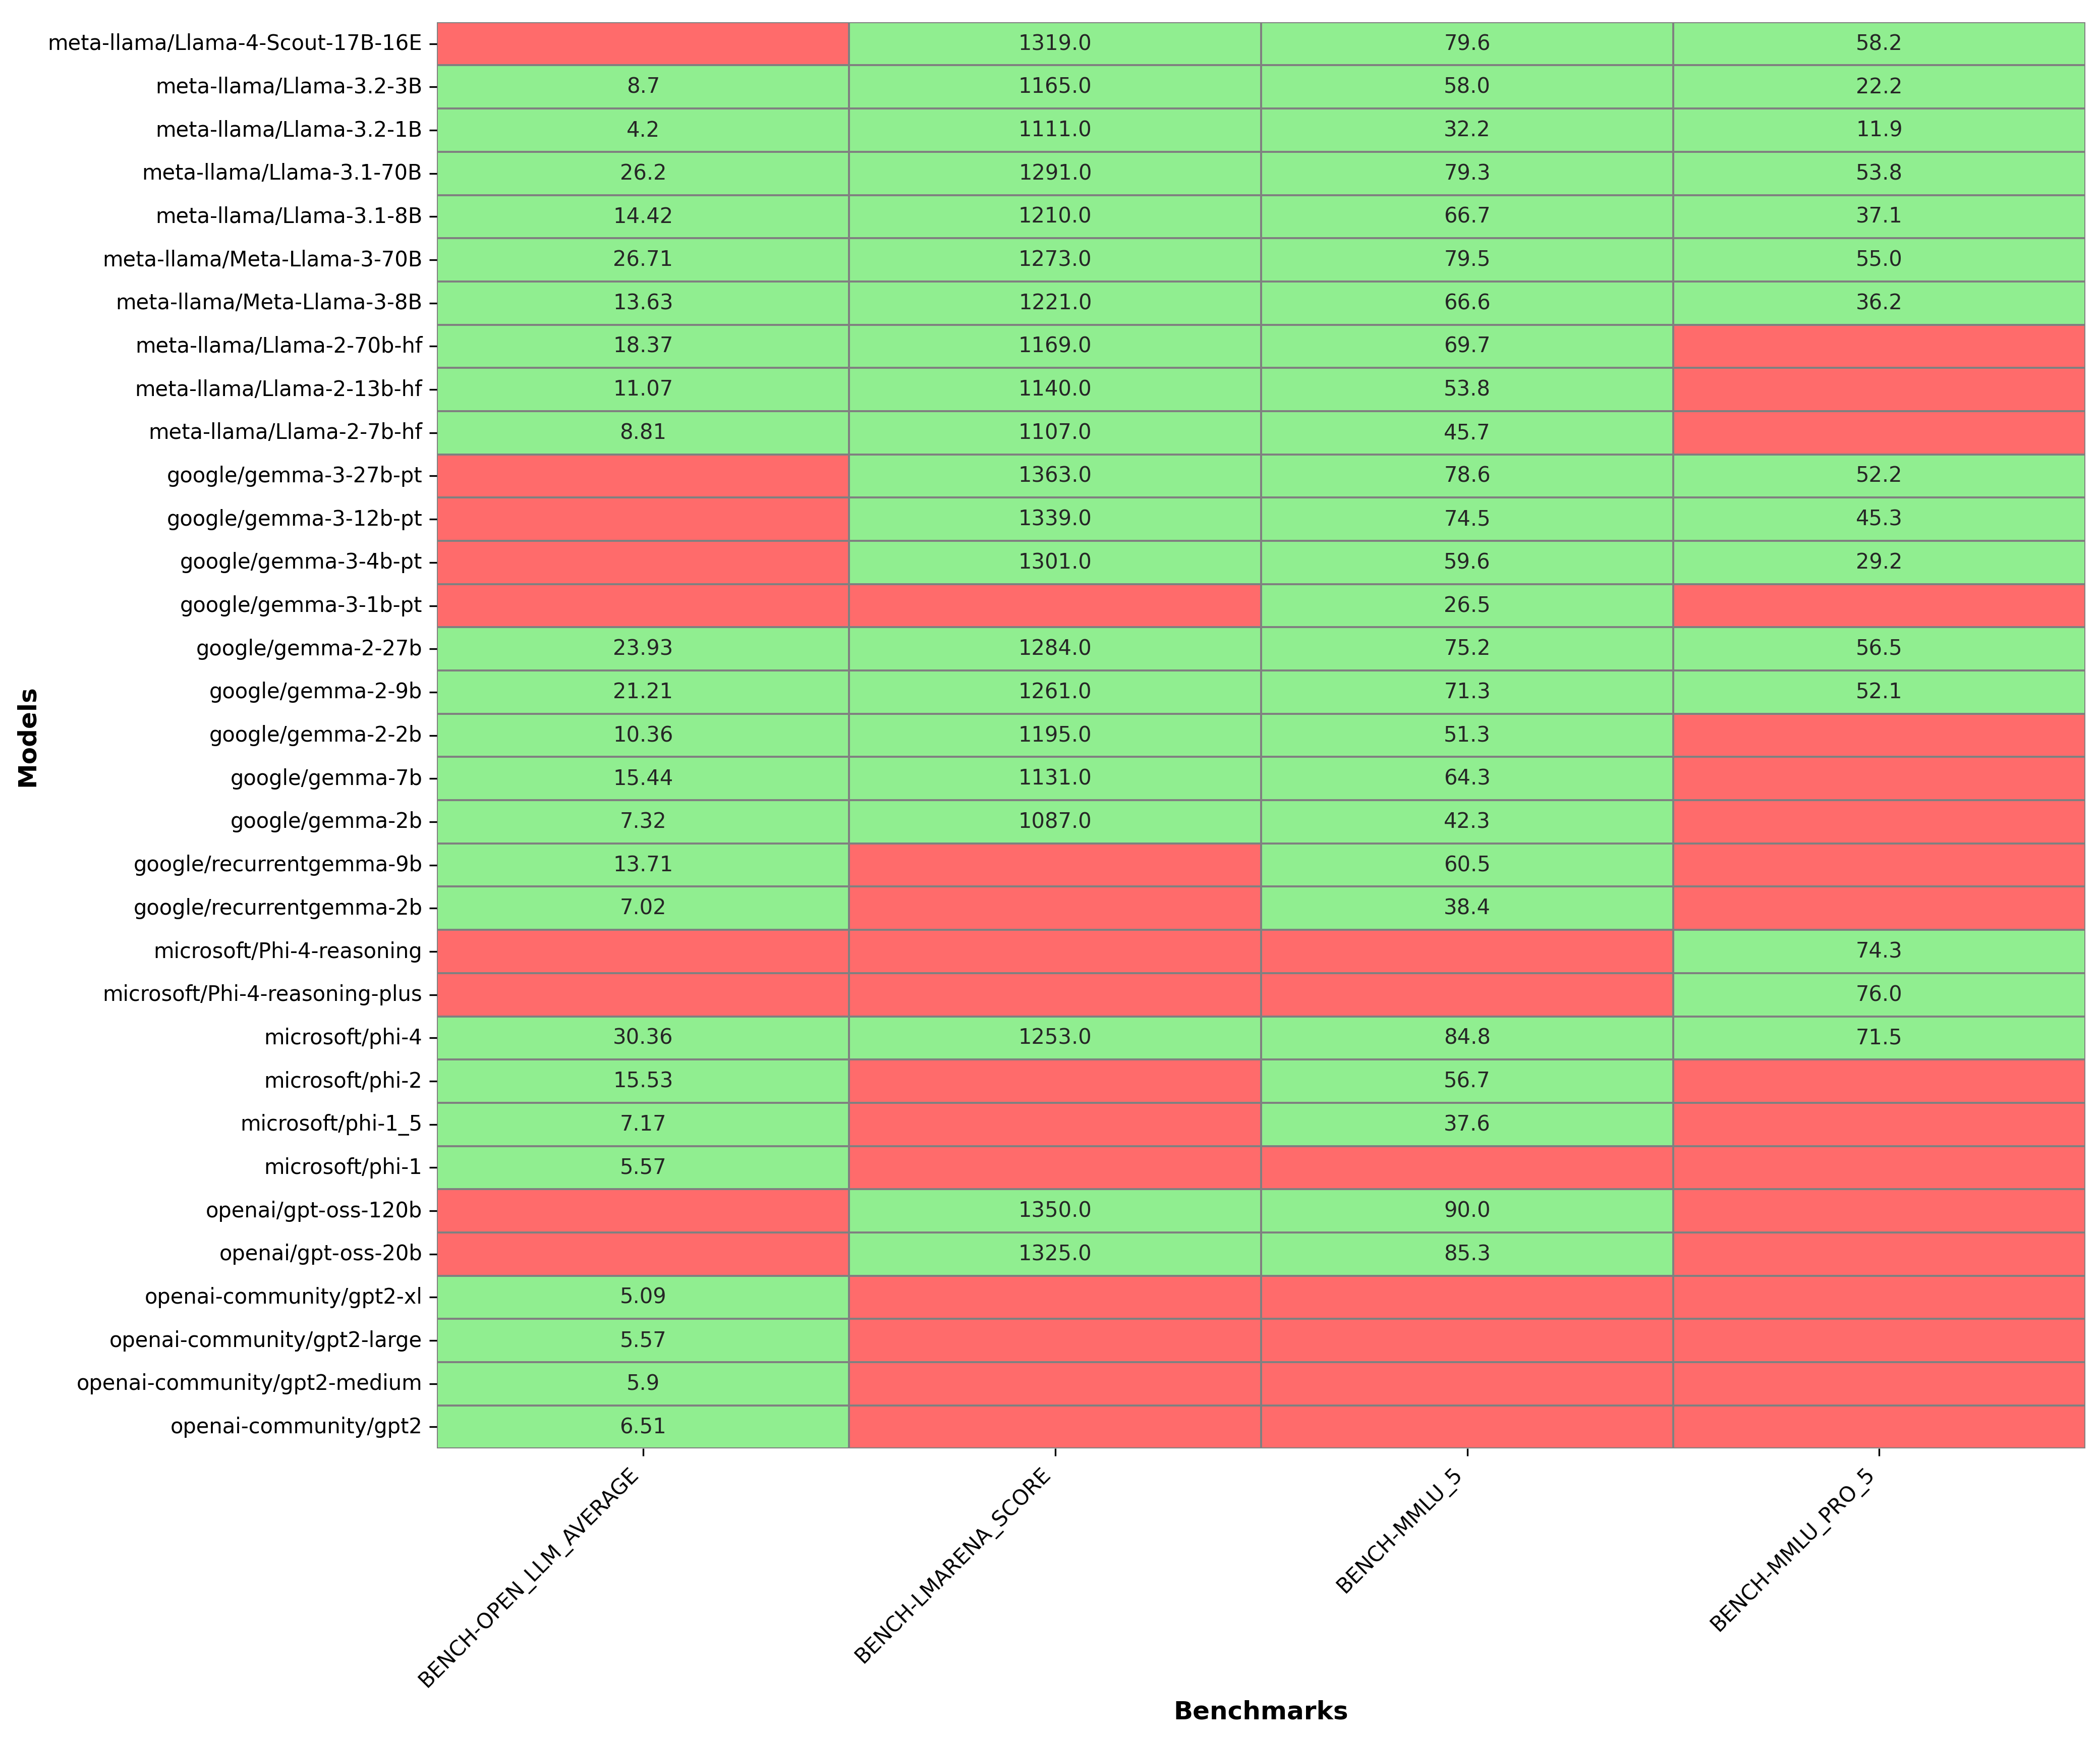
\includegraphics[width=\linewidth]{img/benchmark_availability.png}
            \caption{Availability of benchmark results for the selected models.}
            \label{fig:benchmark_availability}
        \end{figure}

\subsection{Comparing LMC Complexity and Inference Capability}


